\section{Rotation3DMatrix Class Reference}
\label{classRotation3DMatrix}\index{Rotation3DMatrix@{Rotation3DMatrix}}
{\tt \#include $<$rotation3dmatrix.h$>$}

Inheritance diagram for Rotation3DMatrix::\begin{figure}[H]
\begin{center}
\leavevmode
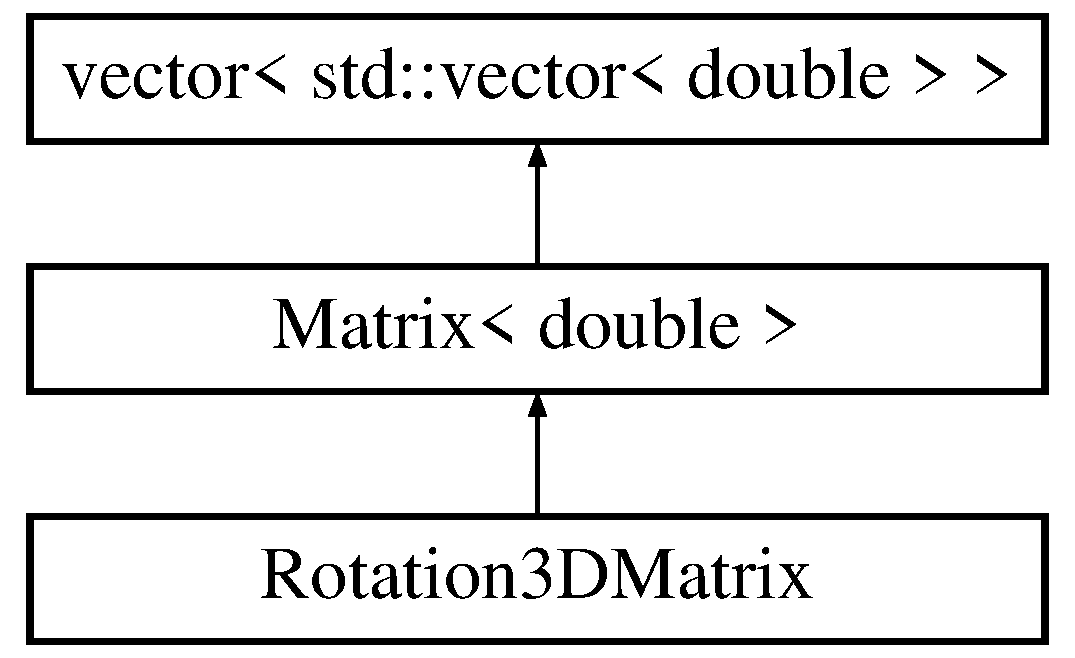
\includegraphics[height=3cm]{classRotation3DMatrix}
\end{center}
\end{figure}
\subsection*{Public Methods}
\begin{CompactItemize}
\item 
{\bf Rotation3DMatrix} (double x\-Corner, double y\-Corner, double z\-Corner)
\end{CompactItemize}


\subsection{Constructor \& Destructor Documentation}
\index{Rotation3DMatrix@{Rotation3DMatrix}!Rotation3DMatrix@{Rotation3DMatrix}}
\index{Rotation3DMatrix@{Rotation3DMatrix}!Rotation3DMatrix@{Rotation3DMatrix}}
\subsubsection{\setlength{\rightskip}{0pt plus 5cm}Rotation3DMatrix::Rotation3DMatrix (double {\em x\-Corner}, double {\em y\-Corner}, double {\em z\-Corner})\hspace{0.3cm}{\tt  [inline]}}\label{classRotation3DMatrix_a0}




The documentation for this class was generated from the following file:\begin{CompactItemize}
\item 
{\bf rotation3dmatrix.h}\end{CompactItemize}
